\chapter{Simulating interaction between CSF and the Spinal Cord}
The previously described model is used on a different geometry based on idealized versions of the spinal cord. The meshes have the same dimensions as found in previous work by Dr{\o}sdal, \cite{Dros11} except for the size of the syrinx which is increased from 1 mm to 3 mm in diameter. 
\\
\\
\\
\section{Overview of previous studies}
To our knowledge, few studies has investigated fluid-structure interaction modeling of the CSF and the spinal cord including a syrinx. The spinal cord has fibres oriented in the axial direction and a direction-dependent Youngs modulus would then be expected. 

In the literature values range between 0.012 to 1.98 MPa. As reported by \cite{Clar10} most of spinal cord experimental studies use a tensile test, and the stress-strain and stress-relaxation responses of the spinal cord are non-linear. Therefore, it will in general be hard to compare results from different studies using different arbitrary levels of strain. Another approach used by Kwon \cite{Kwon02}, focuses more on spinal cord injuries and are thus more interested in properties during compression. From the modeling point of view, both approaches is of interest, and better constitutive models could be attained by combining results from several of these studies. In this work, however, we limit Youngs modulus to be a constant independent of spatial direction. Such an assumption has been made in all the previous cited works in this thesis. 
\\
\\
Some studies have investigated the effects of FSI on the spinal cord movement and CSF pressure in geometries without a syrinx. Clark \cite{Clar13} assumed the Youngs modulus to be 1 MPa for the spinal cord, and in their initial tests this choice caused only small displacements. Therefore the conclusion was that FSI had a negligible effect on CSF pressure in the SAS. \\
Cheng et al. \cite{Chen14} investigated FSI effects on a patient-specific 3D-geometry. In their model they assumed a Youngs modulus of 0.7 MPa, and reached the same conclusion as Clark. As highlighted: \textit{"This study informs that fluid structure interaction has no effect on CSF pressure"}. 
\\ Clearly, a too high elastic modulus will undermine the effects of FSI, if they do exist. Considering the wide range of material parameters reported in the literature for the spinal cord, we believe further investigation is necessary to be able to make such a statement. In addition, these two studies does not seem to investigate syringomelia as a primary target, and therefore important effects of FSI could have been overlooked in these specific cases. \\
\\
\\
In porous models presented by Dr{\o}sdal, \cite{Dros11} fluid pressure within the cord was altered by the presence of a syrinx but the CSF pressure in the SAS was not. velocities up to only 3e-7 cm/s inside the syrinx was reported, and therefore there must be some other effects causing the more rapid fluid movement inside the syrinx.  
\\
\\
To our knowledge, the most noted group working on FSI effects on Syringomelia include the group of Chris D. Bertram at the University of Sydney. Some of their work include research on pressure waves propagating in the spinal cord in the presence of a syrinx \cite{Bert05},\cite{Bert08},\cite{Bert09}. Even though, in this specific paper Bertram focuses on the overlap between the cervical and thoracic segments of the spinal cord, the mechanisms of interest remians the same,
\\
\\
xxx Move to medical section? xxx namely the 'slosh' mechanism proposed by Williams in 1980 \cite{Will80}. In this theory, increased CSF pressure in the SAS is transmitted to the syrinx generating waves along the walls. Compression of the upper part of the syrinx results in a downwards displacement of the lower part resulting in enlargement of the syrinx. 
\\
\\
Even with today's high quality magnetic resonance imaging, (MRI) or phase contrast MR (PC-MR), exact velocities are hard to measure. Healthy subjects also has very complex CSF flow and thus difficult to observe or quantify. Since the Chiari I malformation is associated with abnormal CSF flow, a realistic model simulating the pre-operative case needs abnormal inflow or pressure boundary conditions. The latter is extremely hard to measure exact. 


\subsection{Pressure measurements in patients with syringomelia}
Williams (1981) \cite{Will81} and H{\"a}ck (2001) \cite{Hack01} investigated the pressure gradient between the intracranial and spinal (lumbar) CSF compartments. In their work the pulsatile pressure were not analyzed, which seem to be more reliable in predicting intracranial compliance according to more recent studies by Eide \cite{Eide11_Rand,Eide10_Amp,Eide11_Hyper,Eide10_Diag}.
Fri{\v{c}} and Eide also measured the pulsatile pressure gradient between the to compartements and have found significantly higher (mean wave amplitude, MWA) gradients in patients with evidence of syringomyelia (12/26 patients) than in those without. ($3.7 \pm 2.0 \text{ mmHg vs } 2.1 \pm 1.3 \text{ mmHg}; p=0.02$) \cite{Fric15}. See figure \ref{fig:Syrinx} for a graphical representation. 
\begin{center}
\begin{figure}[!ht]
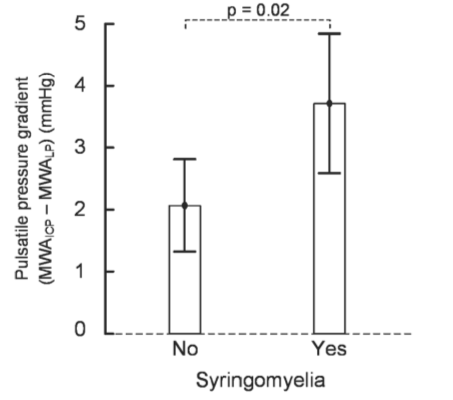
\includegraphics[width=0.4\linewidth]{figures/Eide_pressure_Syrinx}
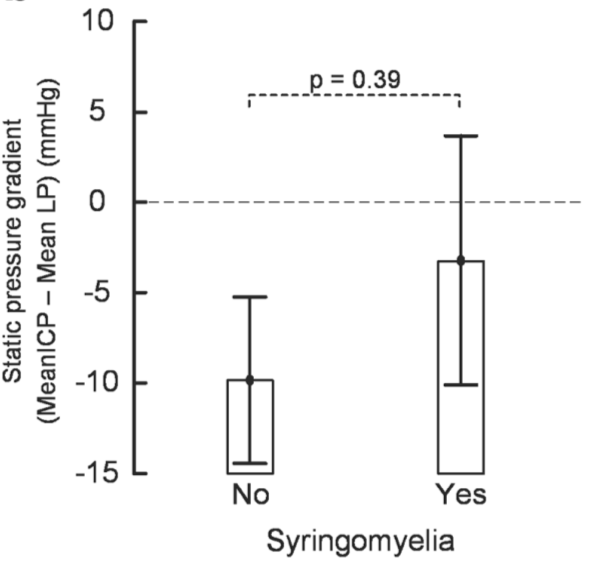
\includegraphics[width=0.375\linewidth]{figures/Eide_static}
\caption{Pulsatile (left) and static pressure gradient in patients as used in the study by Fri{\v{c}} and Eide \cite{Fric15}}\label{fig:Syrinx}
\end{figure}
\end{center}
The pulsatile intracranial pressure (ICP) as well as pulsatile pressure gradients were clearly abnormal or with boarderline values in 69 and 71 \% of Chiari I patients, respectively. Without any further speculation, it is interesting to note that these numbers are very close to the number of Chiari I patients that develops a syrinx. The median pressure difference in patients with abnormal pressure gradient were $2.6$ mm Hg between the intracranial CSF pressure and the lumbar CSF pressure. The actual mean static ICP was measured to a median of $7.1$ mmHg for the patients (range -0.7 -- 13.0), whereas the median of the mean lumbar pressure LP in the patients were $15.1$ mm Hg. Czosnyka and Pickard \cite{Czos04} reported ICP for healthy adult subjects to be $7-15$ mm Hg. Williams \cite{Will76} measured pressure up to $70$ mm Hg and $97$ mmHg in the SAS in the cisternal (just below the cerebellum) and lumbar region, respectively during coughing. Sansur et al. \cite{Sans03} measured the SAS pressure at the L5-level and found pressures up to $125$ mm Hg in patients coughing. The baseline pressures for healthy subjects were reported to be 8.6 -- 13.4 mm Hg.  
\\
\\
\begin{center}
\begin{figure}[!ht]
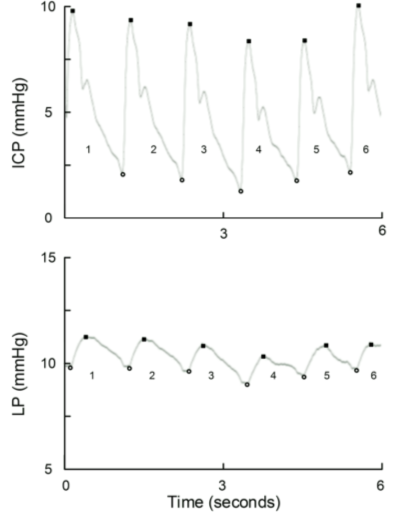
\includegraphics[scale=0.5]{figures/ICP_and_LP}
\caption{Intracranial (ICP) and lumbar (LP) pressure measured simultaneuously by Fri{\v{c}} and Eide}
\end{figure}
\label{fig:ICP_and_LP}
\end{center}
From the modeling point of view, these measurements are of high interest in prescribing the correct boundary conditions at the top and bottom of the cord and SAS model. There are some challenges however. (Discuss pressure measurements in \cite{Fric15}, pressure is always higher in lumbar than in Intracranial)
\\
\\
(Comment on experiments by Martin et al. \cite{Mart09Syrinx})


\section{Assessment of CSF velocities before and after decompression surgery}
We hypothesized that FSI-effects (deformation and pressure wave propagation) was at least partially responsible for the flow up to 3 cm/s within the syrinx as reported by Brucker and Haughton in an assessment of CSF velocities and Cord Motion Before and After Chiari 1 Decompression. The study focused on the upper region (C1-C5) of the spinal cord.

xxx ALSO READ 5, 13, 21, 45 from Karen xxx
\begin{center}
\begin{figure}[!ht]
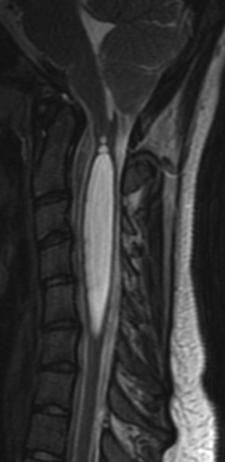
\includegraphics[width=0.51\linewidth]{figures/Syrinx_Subject} 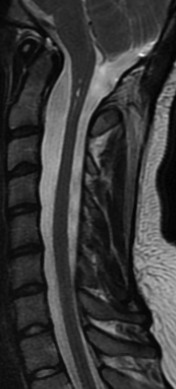
\includegraphics[width=0.474\linewidth]{figures/Syrinx_PostOp}
\centering{\caption{MRI image of 14 year old female subject before and 10 months after decompression. Note the withdrawal of the cerebellar tonsils in the post-operative image on the right}}
\end{figure}
\end{center}
CSF flow was measured with PCMR on three different stages: Pre-operative, 2 months post-operative and 10 months post-operative when the patient had no remaining symptoms. (Add (weighted?) velocity profiles)
 


\begin{figure}[!ht]
\begin{center}
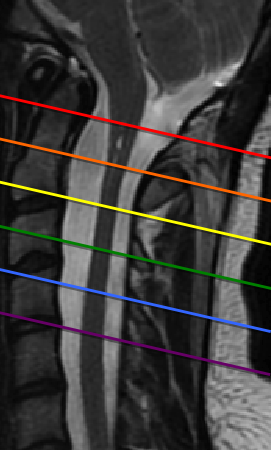
\includegraphics[scale=0.6]{figures/Syrinx_Levels} \\
\caption{Levels C1-C2, C2, C2-C3, C3, C3-C4 and C4-C5}
\end{center}
\end{figure}

\section{Linear Results}
For all Spinal Cord simulations we apply pressure boundary conditions on the inlet and outlet as described under Womersley Flow in chapter 4. First, a sinusodial varying pressure was applied to the boundaries with a maximum of 20 Pa difference between top and bottom. This applied pressure gradient has previously been reported to result in peak velocities of around 6 cm/s assuming a rigid, but porous cord. \cite{Dros11} The Simulations were run 10 cycles where a steady state was reached. Quantities of interest are the peak velocity in the SAS, max$|\mathbf{v}|$, the peak velocity inside the syrinx in the spinal canal, max$|\mathbf{v}_{sc}|$ and the maximum displacemen,t max$|\mathbf{U}|$ in both x- and y-direction.
\\
\\
\begin{table}[!ht]
\begin{center}
  \begin{tabular}{l | l | l | l | l | l | l }
    $N_x$ & $N_y$ & dofs & max$|\mathbf{v}|$[cm/s] & max$|\mathbf{v}_{sc}|$[cm/s] & max$|\mathbf{U}_x|$[mm] & max$|\mathbf{U}_y|$[mm] \\ \hline
    18  & 30 & 6281 & 6.11 & 0.79 & 0.34 & 0.07 \\ \hline
	36  & 60 & 24437 & 6.02 & 0.83 & 0.33 & 0.02 \\ \hline
    \hline
  \end{tabular}
  \end{center}
  \caption{$E = 16 kPa, \Delta t = 0.002s, T = 10, \rho_s = 2\rho_f$}
\end{table}

\begin{table}[!ht]
\begin{center}
  \begin{tabular}{l | l | l | l | l | l | l }
    $N_x$ & $N_y$ & dofs & max$|\mathbf{v}|$[cm/s] & max$|\mathbf{v}_{sc}|$[cm/s] & max$|\mathbf{U}_x|$[mm] & max$|\mathbf{U}_y|$[mm] \\ \hline
    18  & 30 & 6281 & 7.75 & 2.30 & 1.30 & 0.16 \\ \hline

    \hline
  \end{tabular}
  \end{center}
  \caption{$E = 5 kPa, \Delta t = 0.002s, T = 10s, \rho_s = 2\rho_f$}
\end{table}

\section{Nonlinear Results}
New simulations. Non-linear addition in both $\sigma$ and convection. $\rho_s =1.75 \rho_f$
Else, same
\begin{table}[!ht]
\begin{center}
  \begin{tabular}{l | l | l | l | l | l | l }
    $N_x$ & $N_y$ & dofs & max$|\mathbf{v}|$[cm/s] & max$|\mathbf{v}_{sc}|$[cm/s] & max$|\mathbf{U}_x|$[mm] & max$|\mathbf{U}_y|$[mm] \\ \hline
    18  & 30 & 6281 & 7.10 & 2.28 & 0.96  & 0.06 \\ \hline
	36 & 60 & 24437 & 6.71 & 2.07 & 0.86 & 0.06 \\ \hline

    \hline
  \end{tabular}
  \end{center}
  \caption{$E = 5 kPa, \Delta t = 0.002s, T = 10s, \rho_s = 1.75 \rho_f$}
\end{table}

\begin{table}[!ht]
\begin{center}
  \begin{tabular}{l | l | l | l | l | l | l }
    $N_x$ & $N_y$ & dofs & max$|\mathbf{v}|$[cm/s] & max$|\mathbf{v}_{sc}|$[cm/s] & max$|\mathbf{U}_x|$[mm] & max$|\mathbf{U}_y|$[mm] \\ \hline
    18  & 30 & 6281 & 5.93 & 0.96 & 0.35 & 0.02 \\ \hline

    \hline
  \end{tabular}
  \end{center}
  \caption{$E = 16 kPa, \Delta t = 0.002s, T = 10, \rho_s = 2\rho_f$}
\end{table}

